\exercise

Given zdelta’s approach to compressing pairs of files,
%
\begin{enumerate}

  \item describe how zdelta works by assuming that $f_{known} = \text{\tt
  babbo}$ and $f_{new} = \text{\tt nababbi}$;

  \item let us assume that you are given 5 strings $S = \{ \text{\tt abaco},
  \text{\tt baxco}, \text{\tt taco}, \text{\tt zaxo} \}$, describe how zdelta
  compresses these files via a properly constructed weighted directed graph.

\end{enumerate}

\solution

\begin{enumerate}

  \item  The compression produces the following tuples:
  %
  \begin{table}[H]
    \centering
    \begin{tabular}{r|lcl}
    {\tt b a b b o} & \colorbox{yellow}{\tt n} {\tt a b a b b i \$} & &
    $\langle 0, 0, \text{\tt n} \rangle$ \\
    {\tt b} \colorbox{pink}{\tt a b} {\tt b o} & {\tt n}
    \colorbox{yellow}{\tt a b a} {\tt b b i \$} & &
    $\langle 5, 2, \text{\tt a} \rangle$ \\
    {\tt b a} \colorbox{pink}{\tt b b} {\tt o} & {\tt n a b a}
    \colorbox{yellow}{\tt b b i} {\tt \$} & &
    $\langle 7, 2, \text{\tt i} \rangle$ \\
    {\tt b a b b o} & {\tt n a b a b b i} \colorbox{yellow}{\tt \$} & &
    $\langle 0, 0, \text{\tt \$} \rangle$ \\
    \end{tabular}
  \end{table}

  \item The graph can be represented as an adjacency matrix, where each cell
  $(r, c)$ contains the number of tuples produced by $gzip(s_c \mid s_r)$ (i.e.,
  the compression of $s_c$ given $s_r$).
  %
  \begin{table}[H]
    \centering
    \begin{tabular}{c|c|c|c|c|}
      & {\tt abaco} & {\tt baxco} & {\tt taco} & {\tt zaxo} \\ \hline
      $\varepsilon$ & 5 & 6 & 5 & 5 \\ \hline
      {\tt abaco} & - & 2 & 2 & 3 \\ \hline
      {\tt baxco} & 3 & - & 3 & 3 \\ \hline
      {\tt taco} & 2 & 3 & - & 3 \\ \hline
      {\tt zaxo} & 3 & 3 & 3 & - \\ \hline
    \end{tabular}
  \end{table}
  %
  A possible MST may be:
  %
  \begin{figure}[H]
    \centering
    \tikzstyle{level 1}=[level distance=3cm, sibling distance=2cm]
    \tikzstyle{level 2}=[level distance=3.5cm, sibling distance=1cm]
    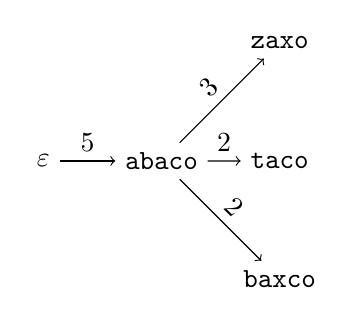
\begin{tikzpicture}[grow=right, sloped]
    \node[draw=none,fill=none] {$\varepsilon$}
        child {
            node[draw=none,fill=none] {\tt abaco}
                child {
                    node[draw=none,fill=none] {\tt baxco}
                    edge from parent[->]
                    node[above] {2}
                }
                child {
                    node[draw=none,fill=none] {\tt taco}
                    edge from parent[->]
                    node[above] {2}
                }
                child {
                    node[draw=none,fill=none] {\tt zaxo}
                    edge from parent[->]
                    node[above] {3}
                }
                edge from parent[->]
                node[above] {5}
        };
    \end{tikzpicture}
  \end{figure}

\end{enumerate}
